\documentclass[border=3pt]{standalone}
\usepackage{mathptmx}
\usepackage{tikz}
\usetikzlibrary{positioning,arrows.meta,fit,calc,decorations.pathreplacing,backgrounds}
\definecolor{cblue}{HTML}{2A78D6}\definecolor{corange}{HTML}{EB6834}\definecolor{caqua}{HTML}{1BAF7A}
\definecolor{ink}{HTML}{0B0B0B}\definecolor{ink2}{HTML}{52514E}\definecolor{muted}{HTML}{8A8984}\definecolor{fillg}{HTML}{F3F2EE}
\definecolor{fblue}{HTML}{DBE8F8}\definecolor{forange}{HTML}{FDE3D8}
\begin{document}
\hyphenpenalty=10000 \exhyphenpenalty=10000 \frenchspacing
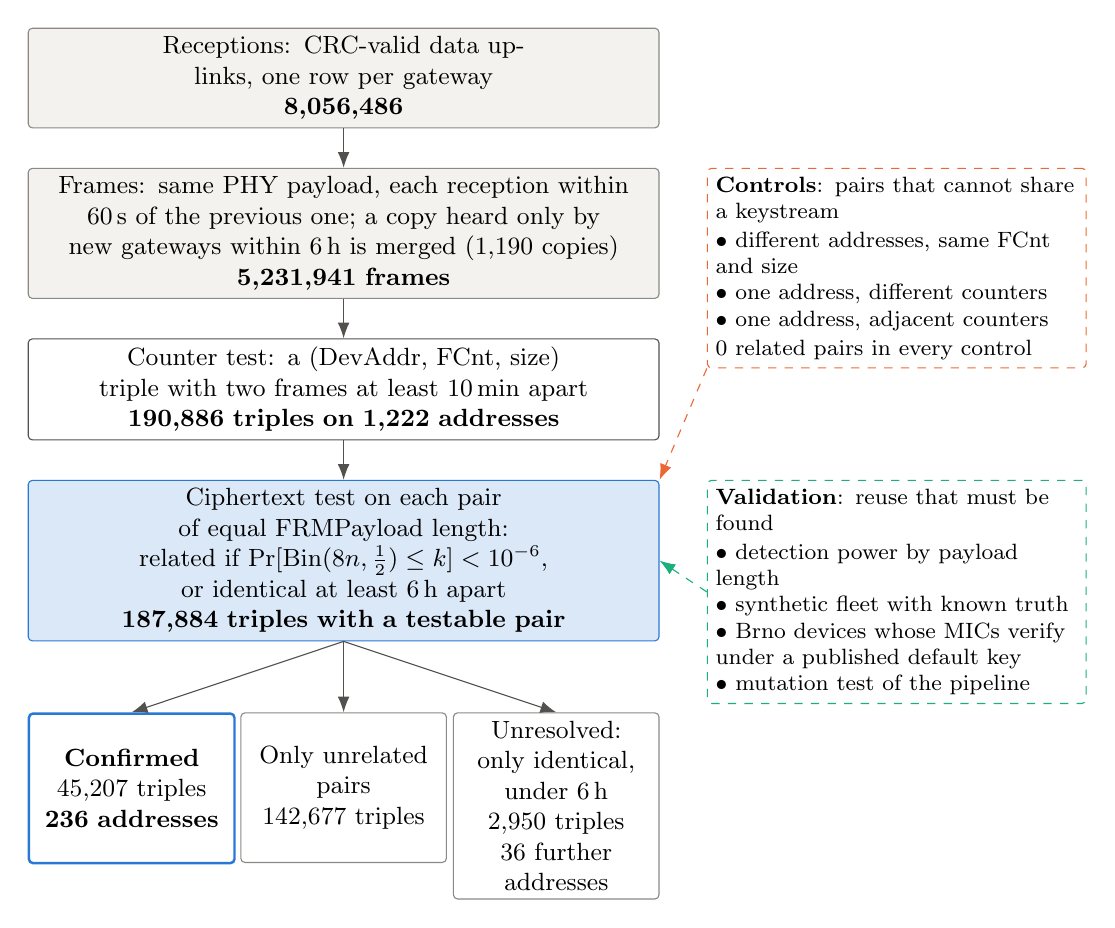
\begin{tikzpicture}[font=\small, >={Latex[length=2mm]}, node distance=5mm,
  st/.style={draw=muted, fill=fillg, rounded corners=1.5pt, align=center, text width=78mm, inner sep=3pt, minimum height=11mm},
  res/.style={draw=muted, rounded corners=1.5pt, align=center, text width=24mm, inner sep=3pt, minimum height=19mm},
  side/.style={rounded corners=1.5pt, dashed, align=left, text width=46mm, inner sep=3pt, font=\footnotesize},
  num/.style={font=\small\bfseries}]
\node[st] (rec) {Receptions: CRC-valid data uplinks, one row per gateway\\ {\bfseries 8,056,486}};
\node[st, below=of rec] (frm) {Frames: same PHY payload, each reception within 60\,s of the previous one; a copy heard only by new gateways within 6\,h is merged (1,190 copies)\\ {\bfseries 5,231,941 frames}};
\node[st, fill=white, draw=ink2, below=of frm] (ctr) {Counter test: a (DevAddr, FCnt, size) triple with two frames at least 10\,min apart\\ {\bfseries 190,886 triples on 1,222 addresses}};
\node[st, fill=fblue, draw=cblue, below=of ctr] (cip) {Ciphertext test on each pair of equal FRMPayload length:\\ related if \mbox{$\Pr[\mathrm{Bin}(8n,\frac12)\le k] < 10^{-6}$},\\ or identical at least 6\,h apart\\ {\bfseries 187,884 triples with a testable pair}};
\draw[->, ink2] (rec) -- (frm); \draw[->, ink2] (frm) -- (ctr); \draw[->, ink2] (ctr) -- (cip);
\node[res, draw=cblue, line width=0.9pt, below=9mm of cip.south west, anchor=north west] (o1) {{\bfseries Confirmed}\\ 45,207 triples\\ {\bfseries 236 addresses}};
\node[res, below=9mm of cip.south, anchor=north] (o2) {Only unrelated\\ pairs\\ 142,677 triples};
\node[res, below=9mm of cip.south east, anchor=north east] (o3) {Unresolved: only identical, under 6\,h\\ 2,950 triples\\ 36 further addresses};
\foreach \o in {o1,o2,o3} \draw[->, ink2] (cip.south) -- (\o.north);
\node[side, draw=corange, right=6mm of frm.north east, anchor=north west] (ctl) {{\bfseries Controls}: pairs that cannot share a keystream\\[1pt]
  $\bullet$ different addresses, same FCnt and size\\ $\bullet$ one address, different counters\\ $\bullet$ one address, adjacent counters\\[1pt] 0 related pairs in every control};
\node[side, draw=caqua, right=6mm of cip.north east, anchor=north west] (val) {{\bfseries Validation}: reuse that must be found\\[1pt]
  $\bullet$ detection power by payload length\\ $\bullet$ synthetic fleet with known truth\\ $\bullet$ Brno devices whose MICs verify under a published default key\\ $\bullet$ mutation test of the pipeline};
\draw[->, corange, dashed] (ctl.south west) -- (cip.north east);
\draw[->, caqua, dashed] (val.west) -- (cip.east);
\end{tikzpicture}
\end{document}
